% 模型图
\begin{figure}[htbp]
    \centering
    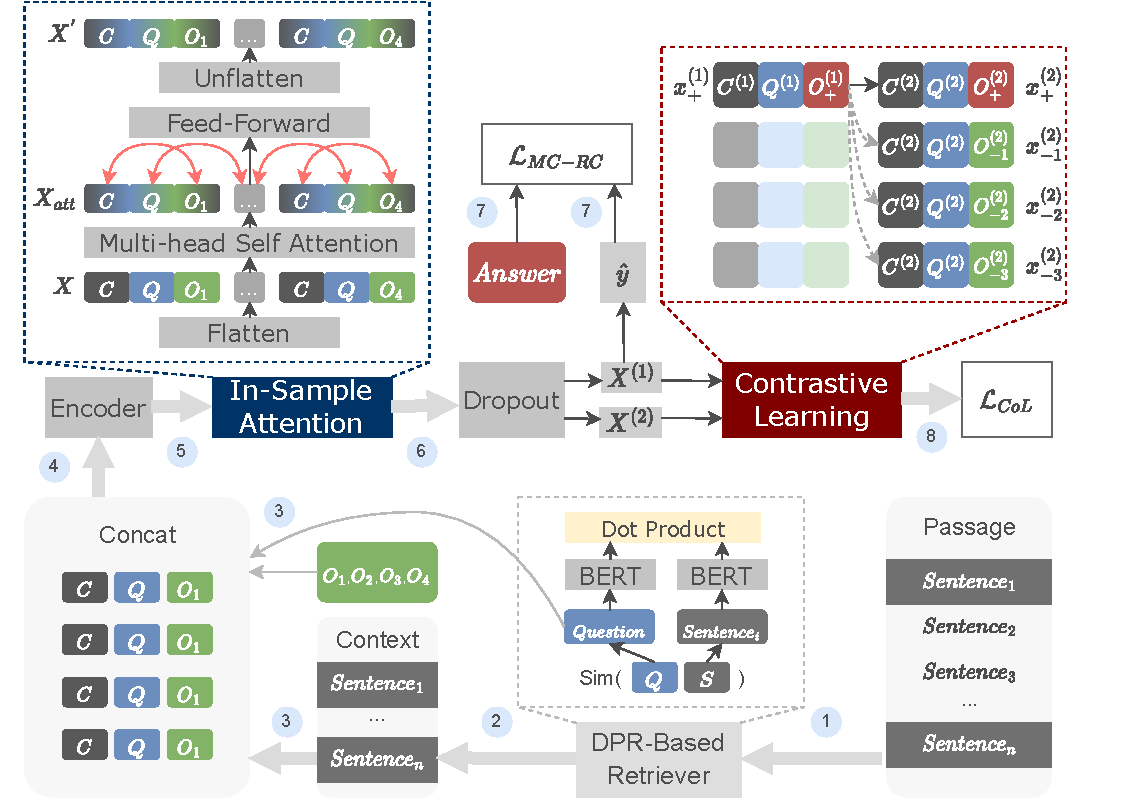
\includegraphics [width=1.0\textwidth] {figure/4-1.pdf}
    % \caption{The architecture of our model CoLISA. (1) A long passage is fed into the DPR-based retriever, (2) then comes out a shorter context, (3) together with a related question and multiple options in our dataset, they are (4) preprocessed and combined into four different sequences (in our dataset there are four options for each question), after going through the inherent (5) embedding and (6) encoder, these four sequences are represented as (7) vector representations, (8) followed by an ISA module listed on the right top of the figure, the sequences are flattened to a combined one, with multi-head self-attention across each token within the extended sequence, then the sequence roll back to the initial dimension, (9) the updated vectors are fed into a dropout twice to come out into two outputs, (10) one for calculating the cross-entropy loss (11) meanwhile both of them need feeding to a CoL module illustrated on the left top of the figure, to calculate a contrastive learning loss finally.}
    \caption{CoLISA的基本架构。} % Our proposed contrastive learning method and in-sample attention mechanism are highlighted boldly in dark red and dark blue rectangles, respectively.
    \label{fig:4-1}
\end{figure}
